\documentclass[10pt,a4paper]{article}
\usepackage[utf8]{inputenc}
\usepackage{amsfonts}
\usepackage{amssymb}
\usepackage{float}
\usepackage{gensymb}
\usepackage{graphicx}
\usepackage{hyperref}
\usepackage{wrapfig}
\hypersetup{
    colorlinks,
    citecolor=black,
    filecolor=black,
    linkcolor=black,
    urlcolor=black,
    linktoc=all,
}
\date{}
\title{Paperwork manual}

\begin{document}

\maketitle

\pagebreak

\tableofcontents

\pagebreak

\section{Introduction}

\begin{figure}[H]
	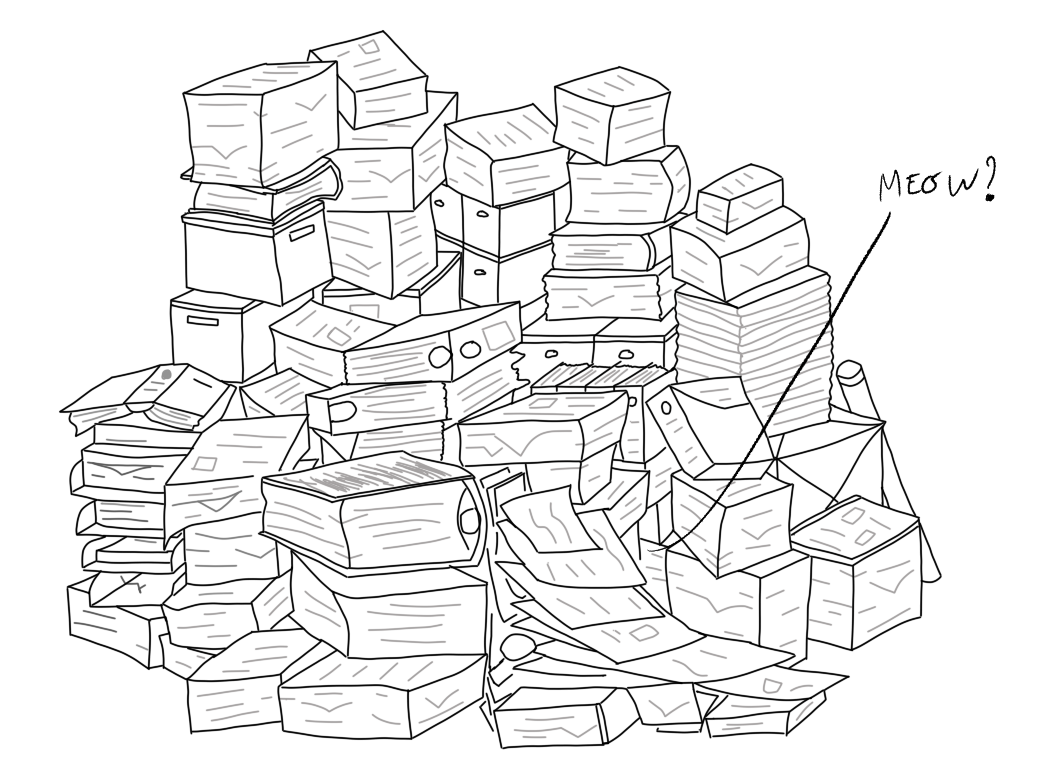
\includegraphics{data/user_manual_intro.png}
\end{figure}

Most personal documents are fairly recurrent: earning statements, rent bills,
electricity bills, etc. For most unorganized people, having to find them back
later is worrisome, at best. For most organized people, naming and sorting them
is as tedious as watching paint dry.

The main idea behind Paperwork is that managing documents is a computer job.
Humans should do as little as possible while machines do most of the work.
The end goal here is "scan \& forget".

If you're looking for a software that will let you name each document
individually, organize them in complex hierachy, tag them manually each time,
fix OCR minor glitches, etc, then Paperwork is not for you.


\section{Definitions}

\subsection{Work directory}

Paperwork stores all your documents in a single directory: the work directory.
In this directory, each document has its own sub-directory.

While this makes Paperwork hard to use with other tools, it has one major
advantage: You don't have to worry about file names and directory structures
anymore.

\subsection{Document}

\begin{figure}[H]
	\includegraphics[scale=0.33]{out/main_window_split.png}
\end{figure}


In Paperwork, a document is a set of pages. On disk, it can either be a set of
JPEG files or a PDF file.

Documents are identified only by a date. It can either be the date you
imported them (default) or some date of your choosing.

They are displayed on the left side of the main window (green part on the
screenshot above).


\subsection{Page}

In Paperwork, a page is just an image and the word positions on this image.

Images can come from a scanner or be imported. In those cases, it is
stored as a JPEG files and text is extracted using OCR (Optical Character
Recognition). OCR is a fairly long process. It can take up to a few minutes for
each page. So the text extracted from images is stored in hOCR files beside
the JPEG files.

Pages can also be the pages from a PDF file. In that case, by default,
Paperwork just stores a copy of the PDF file.

Paperwork does not track whether a page is recto or verso.
Paperwork does not track the paper size corresponding to a page (A4, Letter,
etc).

Pages are displayed on the right side of the main window (blue part on the
screenshot above).


\subsection{Indexation and Keywords}

\begin{figure}[H]
	\includegraphics[scale=0.33]{out/search.png}
\end{figure}

Of course, you need a way to find back your documents. Paperwork manages an
index with all the keywords found in your documents.

Just type in a few keywords, and you will get your documents back.


\subsection{Labels and additional keywords}

\begin{figure}[H]
	\centering
	\begin{minipage}{.5\textwidth}
		\centering
		\includegraphics[scale=0.33]{out/doc_labels.png}
	\end{minipage}%
	\begin{minipage}{.5\textwidth}
		\centering
		\includegraphics[scale=0.33]{out/doc_extra_text.png}
	\end{minipage}
\end{figure}

Unfortunately, sometimes, documents don't contain the keywords needed to find
them back. Also OCR is a perfectly realiable process and may not work.

To mitigate those issues, you can add labels (or tags) on your documents and
provide additional keywords. Both are added to the index.

Labels are displayed beside documents. Additional keywords are almost never
displayed.


\section{Settings}

\subsection{Accessing the settings}

\begin{figure}[H]
	\centering
	\begin{minipage}{.5\textwidth}
		\centering
		\includegraphics[scale=0.33]{out/app_menu.png}
	\end{minipage}%
	\begin{minipage}{.5\textwidth}
		\centering
		\includegraphics[scale=0.5]{out/app_menu_opened.png}
	\end{minipage}
\end{figure}

\begin{figure}[H]
	\includegraphics[scale=0.33]{out/settings.png}
\end{figure}


\subsection{Work directory}

\begin{figure}[H]
	\includegraphics[scale=0.33]{out/settings_storage.png}
\end{figure}

The work directory is the directory where you want all your documents stored.
It can be a standard folder, a folder synchronized across multiple computers
or on a network share.

Once you close the settings dialog, the work directory will be scanned and
Paperwork index will be updated according to its index.

Each time Paperwork starts, it will look for changes in this folder and
synchronize its index accordingly.


\subsection{Scanner}

\begin{figure}[H]
	\includegraphics[scale=0.33]{out/settings_scanner.png}
\end{figure}


\subsubsection{Device}

\begin{figure}[H]
	\includegraphics[scale=0.33]{out/settings_scanner_device.png}
\end{figure}

When starting, Paperwork looks for scanners. The scanner to use can be selected
in the settings.

Webcams, file storage, etc, cannot be used. Only paper-eaters.


\subsubsection{Scan Mode}

\begin{figure}[H]
	\includegraphics[scale=0.33]{out/settings_scanner_mode.png}
\end{figure}

Most modern scanners scan in color in a reasonable time. However some older
scanners scan much faster in grayscale or even in black\&white. Here you can
select the mode to use.


\subsubsection{Scan Resolution}

\begin{figure}[H]
	\includegraphics[scale=0.33]{out/settings_scanner_resolution.png}
\end{figure}

Scanner resolution defines how detailed the images coming from your
scanner must be.

Higher resolutions mean
\begin{itemize}
	\item longer scans,
	\item longer OCR,
	\item more time to display,
	\item more space used on disk,
	\item but also better OCR.
\end{itemize}

Lower resolutions mean
\begin{itemize}
	\item shorter scans,
	\item shorter OCR,
	\item less time to display,
	\item less space used on disk,
	\item but also inferior OCR,
	\item and possibly unreadable image (even by a human).
\end{itemize}

300 dpi is considered a good trade-off. You may want to reduce it
to 200 dpi on slow computers.


\subsubsection{Scanner calibration}

\begin{figure}[H]
	\includegraphics[scale=0.33]{out/settings_calibration_dialog.png}
\end{figure}

Scanners tend to provide images actually bigger than the scanned pages.
Since most of the time, you will always scan pages having the same
size (A4 or Letter usually), Paperwork provides an option called scanner
calibration. Scanner calibration in Paperwork is simply an area that will
always be cropped out of images coming from the scanner.


\subsection{OCR}

\begin{figure}[H]
	\includegraphics[scale=0.33]{out/settings_optical_character_recognition.png}
\end{figure}

By default, Paperwork uses Tesseract for the OCR. If unavailable,
it falls back on Cuneiform.

On Linux, if installed with Flatpak, Paperwork is always provided with
Tesseract. On Windows, Paperwork is always provided with Tesseract.

To get better results, OCR tool need to know the language used in
the document(s).

The language available in the settings dialog of Paperwork are those
understood by the OCR tool. If your language is not in the list, it
means the OCR tool doesn't have the data required to read your language
and you must install them.


\subsubsection{Adding languages}

\paragraph{Flatpak}

\begin{verbatim}
# <langs> is a list of 2-letters language codes separated ';'
# ex: en;fr;de
flatpak config --user --set languages "<langs>"
flatpak update
\end{verbatim}


\paragraph{Debian}

\begin{verbatim}
# <lang> is a 3-letter language code
# ex: 'fra' for French
$ sudo apt-get install tesseract-ocr tesseract-ocr-<lang>
\end{verbatim}

\paragraph{Fedora}

\begin{verbatim}
# <lang> is a 3-letter language code
# ex: 'fra' for French
$ sudo dnf install tesseract tesseract-langpack-<lang>
\end{verbatim}

\paragraph{Ubuntu}

\begin{verbatim}
# <lang> is a 3-letter language code
# ex: 'fra' for French
$ sudo apt-get install tesseract-ocr tesseract-ocr-<lang>
\end{verbatim}

\paragraph{Windows}

Tesseract and all its data files are provided by Paperwork's installer.
You can rerun the installer to install other languages.

If a language is not available in the installer, it either means it
hasn't been packaged (in which case you can request it), or there
is no data file available yet for this language.


\subsubsection{Disabling OCR}

When you scan a page using Paperwork, Paperwork will immediately run
the OCR on it. This process may take a while for each page. In case you want
to scan a lot of pages quickly (for instance, the first time you use
Paperwork), OCR can be temporarily disabled. To disable OCR, you simply have to
unselect all OCR languages.


\subsection{Updates}

\begin{figure}[H]
	\includegraphics[scale=0.33]{out/settings_updates.png}
\end{figure}

If you enable this option, when Paperwork starts, Paperwork will look for
updates if it hasn't done so for a week or more. To know if a new version is
available, it has to send an HTTPS query to 'openpaper.work'.

If an update is found, it will notify you but it won't install it.


\section{New document}

By default, in the document list, Paperwork includes a document called
"New document". If you open it, it always appears empty. This document actually
doesn't exist yet on disk, but will exist as soon as you put a page in it.
You can add pages in it by scanning, importing file(s) or dropping a page from
another in it.

As soon as you put any content in it, this document will get its own date
(the current one by default). In the document list, "New document" will be
replaced by this date, and a new "New document" will be added to the document
list.

\begin{figure}[H]
	\includegraphics[scale=0.33]{out/doc_new_button.png}
\end{figure}

If you are currently searching something (see the chapter "Searching"),
only search results are displayed and therefore this "New document" isn't
displayed. You can get it back by clicking the button "+" in the top left
corner of the main window.


\section{Scanning}

\begin{figure}[H]
	\includegraphics[scale=0.33]{out/page_add.png}
\end{figure}

If a scanner has been selected in the settings, you can use it to scan pages.

In the header bar, there is a button to add pages. The small arrow on the right
gives access to possible page sources. Those page sources include your scanner
sources (Flatbed, Feeder).

Once you've selected the scanner source you want to use, you can click on the
button "Scan from ...".

This will start a scan session:

\begin{itemize}
	\item Scanned pages are appended at the end of the current document.
		If you use a feeder, Paperwork will scan pages until the feeder
		is empty.
	\item Paperwork will then crop them according to scanner calibration.
	\item Paperwork will run OCR on them
	\item Paperwork will index them
\end{itemize}

If this scan session creates a new document, Paperwork will try to set labels
automatically on the document.


\section{Importing}

\begin{figure}[H]
	\includegraphics[scale=0.33]{out/page_add.png}
\end{figure}


\subsection{Images}

Paperwork supports a lot of file formats. It supports JPEG, PNG, GIF,
BMP, TIFF, etc.

Each image file is considered as a page.

Images are always appended to the document currently opened. Simply
select an empty document ("New document") to create a new document while
importing.

OCR is always run on imported images. If the imported image is the
first page of a new document, Paperwork will automatically apply documents
labels.

Note that Paperwork is a document manager. While it can, it is not
designed to handle images with only very little text or photos. Automatic
labeling will not work correctly on such documents.

The OCR (Tesseract) works very well with black text on white background.
Automatic labeling uses recognized text and requires as many keywords
on the first page as possible.


\subsection{PDF}

Each PDF is always considered as a whole document. They are never
appended to existing document. They are copied and renamed in the work
directory, but their content is not modified.
Paperwork always keeps the original PDF file as is, even if you edit some
of its pages: the edited pages are stored beside the PDF file.

Paperwork will look for pages with no text attached. On those pages,
it will automatically run OCR. Once all the pages have been examined,
it will automatically apply document labels. Note that this process
may take a few minutes for big PDFs files.

If the PDF is already part of your documents, Paperwork will simply
ignore it.


\subsection{Many PDFs in one shot}

When importing, if you select a folder, Paperwork will browse this folder and
look for PDFs to import. Already-imported PDFs are simply ignored. Folder
is browsed recursively (all the folders inside the folder are also
examined).


\section{Labels}

\begin{figure}[H]
	\centering
	\begin{minipage}{.5\textwidth}
		\centering
		\includegraphics[scale=0.33]{out/doc_properties_button.png}
	\end{minipage}%
	\begin{minipage}{.5\textwidth}
		\centering
		\includegraphics[scale=0.33]{out/doc_labels.png}
	\end{minipage}
\end{figure}

There is currently one constraint in Paperwork: Each label must be on at least
one document. Otherwise, when you will restart Paperwork, labels without
documents will disappear.


\subsection{Creating new labels}

\begin{figure}[H]
	\includegraphics[scale=0.33]{out/doc_new_label.png}
\end{figure}

You can click on the gray rectangle on the left side to pick the label color.
You can enter the label name in text field between the gray rectangle and
the button "+".

Once you click on the button "+", the label will be added to the current
document.

The label is actually added once you close document properties. Paperwork will
then update its index accordingly.


\subsection{Setting labels on documents}

When you open document properties, the label list appears. On the left side
of each label color, you have a button. This button allows you to add or
remove labels on the current document.

The changes are actually written on disk once you close the document
properties. Paperwork will update its index accordinly.


\subsection{Modifying a label color}

When you open document properties, you can click on a label color to change
it. A dialog will let you pick the new color.

Label color will actually be changed on disk when you close the document
properties. Paperwork will then update the label on all the documents that use
it.


\subsection{Modifying a label name}

When you open document properties, you can click on a label string to change
it. A dialog will let you type in the new name.

Label name will actually be changed on disk when you close the document
properties. Paperwork will then update the label on all the documents that use
it and then reindex them all.


\subsection{Deleting a label}

To the right of each label is white-on-black cross button. Clicking on it
will allow you to delete a label.

Once you will close the document properties, the label will be removed from
all the documents having it. Paperwork will then update its index accordingly.

Beware: Once you have closed document properties, there is no way to put back
the deleted label.


\subsection{Automatic label guessing}

Paperwork does use artificial intelligence. It uses a fairly simple method
actually:
\href{https://en.wikipedia.org/wiki/Naive_Bayes_classifier}{Naive Bayes classifiers}.
It's the same technology used by email clients to classify mails as spam/non-spam.

Based on all the keywords in all your documents that have (or haven't) a label,
it can estimate a probability that a document containing the same keywords
should have or shouldn't have this same label. If the probability is high
enough, it puts the label on the document automatically when you import it or
scan it.

Of course, this approach means that Paperwork needs enough samples to work
reliably. You can expect it to start working once you have about 100 documents
or more (and only for labels that are on more than 10 documents or more).


\section{Searching}

\subsection{Simple search}

\begin{figure}[H]
	\includegraphics[scale=0.33]{out/search.png}
\end{figure}

You simply enter keywords in the search field. In a few seconds, you will get
all the documents containing those keywords.

Paperwork does a "fuzzy" search: documents with keywords close to the one you
gave but not identical are also returned (for instance, 'flech' instead of
'flesch').

You can also use
\href{https://whoosh.readthedocs.io/en/latest/querylang.html}{Whoosh query language}
to make more complex queries. If you want examples, you can use the advanced
search dialog described below.


\subsection{Advanced search}

\begin{figure}[H]
	\centering
	\begin{minipage}{.5\textwidth}
		\centering
		\includegraphics[scale=0.33]{out/advanced_search_button.png}
	\end{minipage}%
	\begin{minipage}{.5\textwidth}
		\centering
		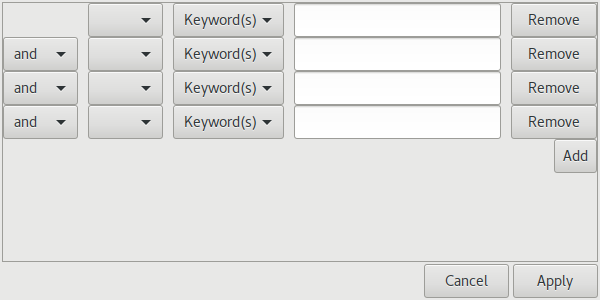
\includegraphics[scale=0.33]{out/advanced_search.png}
	\end{minipage}
\end{figure}

The advanced search dialog helps creating complex search queries. You can
specify various criterias and once you click on the apply button, it will
generate a search query for you and put it immediately in the search field.
Search results will immediately be refreshed as well.


\section{Viewing}

\begin{figure}[H]
	\includegraphics[scale=0.33]{out/docview_layout.png}
\end{figure}

\subsection{Zoom level}

\begin{figure}[H]
	\includegraphics[scale=0.33]{out/docview_layout_scale.png}
\end{figure}

You can change the scale at which pages are displayed using this control.

\subsection{View pages as grid}
\label{layout:grid}

\begin{figure}[H]
	\includegraphics[scale=0.33]{out/docview_layout_grid.png}
\end{figure}

When clicking this button, Paperwork will try to display pages on 3 columns.
In this mode, you can drag'n'drop pages to move them inside the document
or to another document.

\subsection{View pages as list}
\label{layout:paged}

\begin{figure}[H]
	\includegraphics[scale=0.33]{out/docview_layout_paged.png}
\end{figure}

When clicking this button, pages will be scaled so their width is the maximum
width allowed by the main window. In this mode, you can select text in the
page (and then copy it).

\subsection{Highlight all words}

\begin{figure}[H]
	\includegraphics[scale=0.33]{out/docview_layout_show_all_boxes.png}
\end{figure}

This option allows to see quickly all the words identified by OCR. Sometimes
(rarely) OCR misses entire chunk in a page. This option allow to see such
chunk quickly.

\section{Moving pages}

\subsection{Inside a document}

You must display the document pages as a grid (See \ref{layout:grid}).

You can then grab a page (hold the left click button), drag it and drop
it wherever you want in a document. While dragging, a blue marker will show
you where the page would drop if you release the left click button of your
mouse.

\subsection{From a document to another}

You must display the document pages as a grid (See \ref{layout:grid}).

You can then grab a page (hold the left click button), drag it and drop
it in the document list, on the document in which you want the page to go.

\section{Copying text}

\begin{figure}[H]
	\includegraphics[scale=0.33]{out/page_menu_opened.png}
\end{figure}

You must display the document pages as a list (See \ref{layout:paged}).

You can then select text in a page. Hold the left click button to start
selecting, mouse the mouse cursor to select more words, then release it.

You can then copy the selected text, either by pressing Ctrl-C or by using
the page menu at the bottom right of the main window. Once copied, you can
paste the selected text in any other application (Ctrl-V).

\section{Editing a page}

\begin{figure}[H]
	\includegraphics[scale=0.33]{out/page_actions.png}
\end{figure}

Paperwork includes a very simple image editor. It provides 4 functions:

\begin{itemize}
	\item Cropping
	\item Rotating the page by 90\degree (can be rotated multiple times)
	\item Rotating the page by -90\degree (can be rotated multiple times)
	\item Automatic Color Equalization: An algorithm that adjust the image
		brightness, contrast and colors to make it as readable as
		possible.
\end{itemize}

\section{Reseting a page}

Reseting a page returns it to its state when it was scanned or imported,
before any pre-processing did occur.

This can be helpful if you made a bad modification on the page (cropped a wrong
area for instance), if the calibration settings weren't appropriate or if
pre-processing algorithms messed up the page.


\section{Deleting}

When deleting either documents or pages, they are actually moved in the trash
bin of your computer.

\textbf{Important note regarding Flatpak:} A bug may prevent Paperwork from
moving files to the trash (we are working on it). In that case, Paperwork will
delete the file directly (no recovery possible).


\section{Exporting}

You can export both documents or single pages.

In both cases, various transformations can be applied before actually exporting
them. For instance, you can turn color pages into grayscale pages before
putting them in a brand new PDF (making the resulting PDF smaller).


\section{Printing}

You can print both documents or single pages.

Beware that pages are always sent as images to your printer. So for very big
documents, a few minutes may go by before the actual printing start.


\section{Backup}

\section{Synchronisation between multiple computers}

While Paperwork is a personal document manager, it is not a file
synchronization application. They are applications dedicated to file
synchronization that already do that very well. Therefore Paperwork is designed
to be used with such applications (Nextcloud, Dropbox, OneDrive, SparkleShare,
etc).

When you start Paperwork, one of the first things it does is check
the content of the work directory. It looks for any changes and updates
its document list and index accordingly, automatically. So if another instance
of Paperwork on another computer modified something in the work directory
and if this change has been synchronized on another computer, the other
Paperwork will automatically pick up this change when starting.


\subsection{USB key / USB drive}

This is the simplest way to share documents. Simply copy your work directory
to an USB key, tell Paperwork to use it, and you're done.

Beware: You should backup your USB key from time to time on another one.


\subsection{File Synchronization applications}

Those applications synchronize a local directory with a remote server
(or cloud). All the changes you do in your folder are applied on the
server. All the changes applied on the servers are applied to the
computers that connect to it. The server can belong to you or to someone
else (usually a company).

Beware: If you choose to host your documents on someone else server
(DropBox, OneDrive, etc), they can access all your documents. Paperwork
does not encrypt them.

Paperwork is tested daily with Nextcloud. While this is not the easiest one to
install, Nextcloud let you host your files yourself. There are other
self-hosted alternatives that exist: SparkleShare, Syncthing, etc.

Using DropBox or OneDrive can make sense if you're sharing not-so-confidential
documents with others (associations, etc).


\subsubsection{Shared folder}

If all your computers are on the same network, you can share your
work directory. However, be really careful regarding permissions.
Being too permissive could let a pirate access all your personal documents
! And setting them correctly is tricky.

Beware: Using a shared folder means having a single copy of your work
directory. You should do regular backups of your work directory.


\section{Encryption}

\subsection{GNU/Linux}

GNU/Linux distributions include many tools to encrypt whole directories.

With Paperwork, there are 2 directories that should be encrypted to
protect your privacy:
\begin{itemize}
	\item Your work directory (by default \textasciitilde /papers, can be
		changed in the settings)
	\item The cache directory (\textasciitilde /.local/share/paperwork2,
		cannot be changed) (it contains index files from which the
		content of your documents could be partially recovered)
\end{itemize}

Note that if you want to be sure that your data are always encrypted,
it's recommended to encrypt your whole home directory or even your whole system
if possible.

\subsubsection{cryptsetup}

Most GNU/Linux distribution installer now provide an optio4n to encrypt your
whole system or your whole /home with cryptsetup . This is the recommended
method to protect your documents.

\subsubsection{Encfs}

Encfs can also be used to create encrypted directories easily.

Beware that Encfs seems to have some security weaknesses. So, while it's
probably enough to prevent a laptop thief from accessing your documents, it's
likely to be not enough to prevent the NSA or the police from doing so ;-).

\begin{verbatim}
$ encfs ~/.local/share/.paperwork2 ~/.local/share/paperwork2
$ encfs ~/.papers ~/papers
\end{verbatim}


\subsection{Windows}

On Windows, you're strongly advised to enable BitLocker to protect your
documents. If unavailable, there are other applications (Veracrypt, etc).


\section{Keyboard shortcuts}

\begin{figure}[H]
	\includegraphics[scale=0.33]{out/app_menu_opened.png}
\end{figure}

\begin{figure}[H]
	\includegraphics[scale=0.33]{out/shortcuts.png}
\end{figure}

Keyboard shortcuts can be seen by opening the application menu, selecting
"Help" and then "Shortcuts".


\subsection{Paperwork's files locations}

By default:
\begin{itemize}
\item Configuration : \textasciitilde /.config/paperwork2.conf
\item Index : \textasciitilde /.local/share/paperwork2
\item Documents : \textasciitilde /papers
\end{itemize}
(same paths are used on Windows ; \textasciitilde{} = C:\textbackslash Users{[}login{]}
; folders are hidden)

The index is always updated according based on the documents in the
work directory. When Paperwork starts, the modification time of each
file is used to detect changes on the documents.

\subsection{Work directory layout}

workdir|rootdir = \textasciitilde /papers (by default)

\subsubsection{Global organisation}

In the work directory, you have folders, one per document.

The folder names are (usually) the scan/import date of the document:
YYYYMMDD\_hhmm\_ss{[}\_<idx>{]}. The suffix 'idx' is optional and
is just a number added in case of name collision.

In every folder you have:
\begin{itemize}
	\item For image documents:
	\begin{itemize}
		\item paper.$<$X$>$.jpg: The original page in JPG format (X starts at 1)
		\item paper.$<$X$>$.edited.jpg (optional): The page as edited by the user (X starts at 1)
		\item paper.$<$X$>$.words (optional): A hOCR file, containing all the words
		found on the page using the OCR (optional, but required for indexing
		; can be regenerated with the options "Redo OCR").
		\item paper.1.thumb.jpg (optional, generated automatically): A thumbnail
		version of the page (faster to load)
		\item labels (optional): a text file containing the labels applied on this document
		\item extra.txt (optional): extra keywords added by the user
	\end{itemize}

	\item For PDF documents:
	\begin{itemize}
		\item doc.pdf: the document
		\item labels (optional): a text file containing the labels applied on this document
		\item paper.$<$X$>$.edited.jpg (optional): The page as edited by the user (X starts at 1)
		\item extra.txt (optional): extra keywords added by the user
		\item paper.$<$X$>$.words (optional): A hOCR file, containing all the words
		found on the page using the OCR. Some PDF contains crap instead of
			the real text, so running the OCR on them can sometimes be useful.
	\end{itemize}
\end{itemize}

Here is an example a work directory organisation:
\begin{verbatim}
$ find ~/papers
/home/jflesch/papers
/home/jflesch/papers/20130505_1518_00
/home/jflesch/papers/20130505_1518_00/paper.1.jpg
/home/jflesch/papers/20130505_1518_00/paper.1.thumb.jpg
/home/jflesch/papers/20130505_1518_00/paper.1.words
/home/jflesch/papers/20130505_1518_00/paper.2.jpg
/home/jflesch/papers/20130505_1518_00/paper.2.edited.jpg
/home/jflesch/papers/20130505_1518_00/paper.2.words
/home/jflesch/papers/20130505_1518_00/paper.3.jpg
/home/jflesch/papers/20130505_1518_00/paper.3.words
/home/jflesch/papers/20130505_1518_00/labels
/home/jflesch/papers/20110726_0000_01f
/home/jflesch/papers/20110726_0000_01/paper.1.jpg
/home/jflesch/papers/20110726_0000_01/paper.1.thumb.jpg
/home/jflesch/papers/20110726_0000_01/paper.1.words
/home/jflesch/papers/20110726_0000_01/paper.2.jpg
/home/jflesch/papers/20110726_0000_01/paper.2.words
/home/jflesch/papers/20110726_0000_01/extra.txt
/home/jflesch/papers/20130106_1309_44
/home/jflesch/papers/20130106_1309_44/doc.pdf
/home/jflesch/papers/20110726_0000_01/paper.1.thumb.jpg
/home/jflesch/papers/20130106_1309_44/paper.2.edited.jpg
/home/jflesch/papers/20130106_1309_44/paper.2.words
/home/jflesch/papers/20130106_1309_44/labels
/home/jflesch/papers/20130106_1309_44/extra.txt
\end{verbatim}

\subsubsection{hOCR files}

With Tesseract, the hOCR file can be obtained with following command:
\begin{verbatim}
tesseract paper.<X>.jpg paper.<X> -l <lang> hocr && mv paper.<X>.html paper.<X>.words
\end{verbatim}
For example:
\begin{verbatim}
tesseract paper.1.jpg paper.1 -l fra hocr && mv paper.1.html paper.1.words
\end{verbatim}

\subsubsection{Label files}

Here is an example of content of a label file:
\begin{verbatim}
facture,#0000b1588c61 logement,#f6b6ffff0000
\end{verbatim}
It's always \[label\],\[color\]. For a same label, the color should
always be the same.

\subsection{Statistics}

You can get various statistics regarding your documents. Just have
a look at the diagnostic output. Statistics are close to the end
of the output.

\section{Getting support}

A forum dedicated to Paperwork exists:
\href{https://forum.openpaper.work}{https://forum.openpaper.work}.

There is also an IRC channel for live discussions:
\href{https://webchat.freenode.net/}{Freenode}, channel \#openpaperwork

If you have questions regarding Paperwork or simply want to chat, those are
the places to go.

\section{Reporting issues}

If you noticed a bug in Paperwork (and you are sure it's a bug), you can
make a bug report.

\subsection{Bug Tracker}

One way to create bug reports is to create tickets on
\href{https://gitlab.gnome.org/World/OpenPaperwork/paperwork/issues}{Paperwork bug tracker: https://gitlab.gnome.org/World/OpenPaperwork/paperwork/issues}.

This is the recommended way to submit a bug report if you would like to discuss
it with Paperwork developpers.

To make sure you include all the required informations, you can use the
tool integrated in Paperwork (see below).


\subsection{Automatic bug report}

\begin{figure}[H]
	\includegraphics[scale=0.33]{out/bug_report.png}
\end{figure}

Paperwork includes a tool to make reporting bugs easier. It allows you to get
easily all the required information to make a perfect bug report.

All attachments are automatically censored to protect your privacy: Document
contents are blurred in screenshots and logs are censored to remove your user
name.

If the bug you want to report is related scanners, please include
"Scanner info." in the bug report files.


\subsubsection{ZIP file}

You can then obtain a ZIP file with all the data. Please make sure the content
of the ZIP file does not contain private information (it shouldn't, but better
safe than sorry). Then you can add this ZIP file to a ticket on Gitlab.


\subsubsection{Automatic submission}

You can also let the tool submit the bug report to openpaper.work
automatically. In that case, you won't be able to discuss the bug with
developers (or you have to leave a way to contact in the bug report).

If you do, the tool will give you a URL to see the submitted bug report.
This URL is private and shouldn't be shared until you made sure there is no
private information in the bug report. If there are private information,
you can request deletion of the bug report by sending an email to
jflesch@openpaper.work (please specify the private URI in your mail so we can
be sure that you are the one who submitted the bug report).


\section{Uninstalling}

Paperwork can be uninstalled. Uninstalling Paperwork \emph{will never}
remove your work directory or your documents.

\subsection{Windows 10}

Paperwork can be uninstalled as any Windows applications, by going in
Windows Control Panel, clicking on "Applications", finding Paperwork in the
list, and then clicking on "uninstall".

\subsection{GNU/Linux}

If you installed Paperwork using the package manager from your distribution
(the recommended way), the uninstallation method depends on the package
manager.

For instance, on GNU/Linux Debian or GNU/Linux Ubuntu, the following command
will take care of it:

\begin{verbatim}
sudo apt remove --purge paperwork-\*
\end{verbatim}

If you installed it using Flatpak, you can use the following command:

\begin{verbatim}
flatpak --user uninstall work.openpaper.Paperwork
\end{verbatim}

\end{document}
